\section{Status Retrieve Design}
This section describes the design and behavior for querying the status of an archive or retrieve process.

\begin{figure}[H]
    \centering 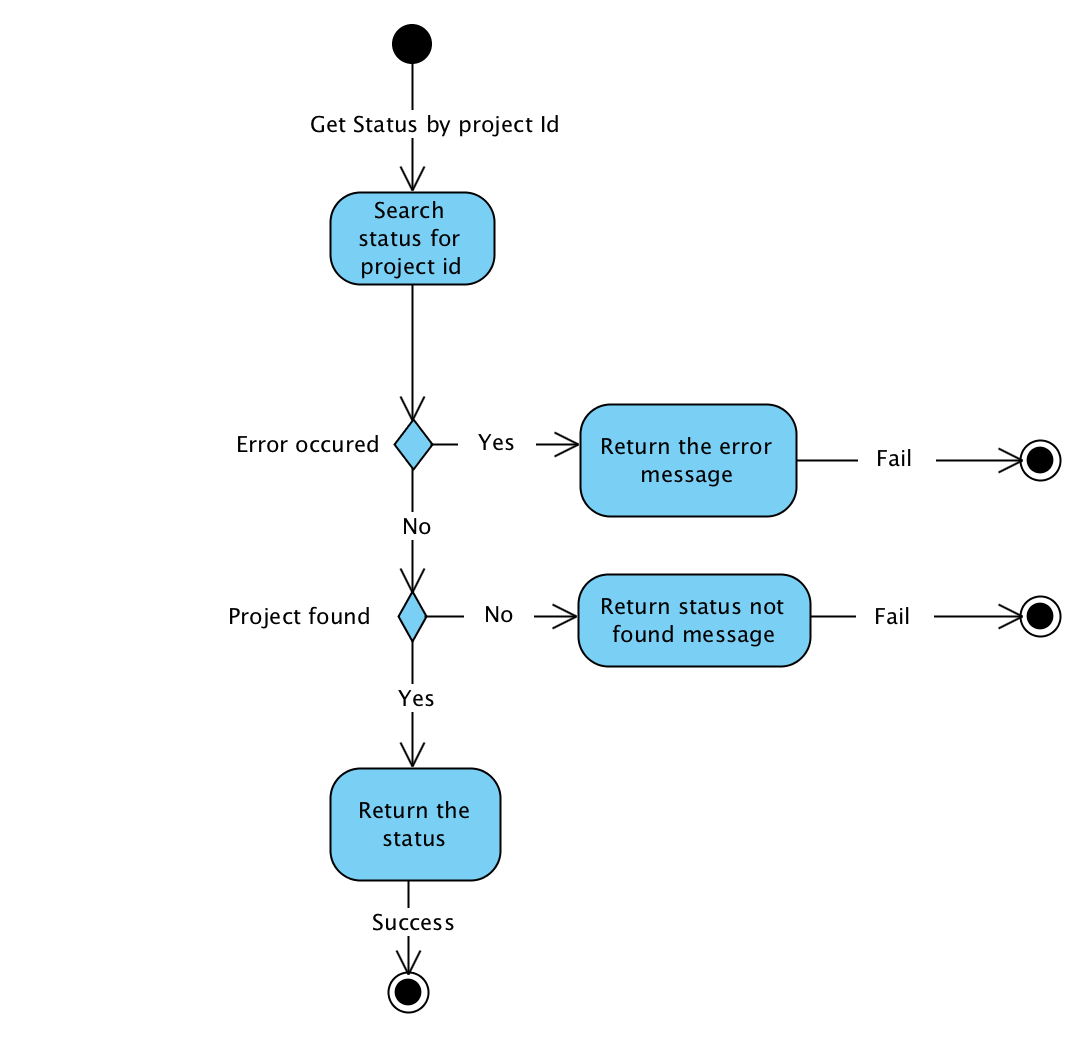
\includegraphics[scale=0.7]{grafiken/activityStatus.png}
    \caption{Activity Diagram of status acknowledgement process}
    \label{fig:activityStatus}
\end{figure}

Figure \ref{fig:activityStatus} illustrates the activity diagram for the status acknowledgement of a project (Listing \ref{lst:status}). Firstly,
the status for the project id is searched and if any error is caught (e.g., unable to connect to database) a message is returned to the client. If the 
status is not found a message stating the "project not found" is sent. Lastly, if the status is found it will be sent to the client.

